\documentclass[main.tex]{subfiles}
\begin{document}

\href{https://www2.seas.gwu.edu/~simhaweb/quantum/modules/module10/module10.html}{Module 10: Algorithms, part I - oracle problems}

\subsection{What is an oracle problem?}
    
    First, the motivation: In the early days of quantum computing, it was not clear that any problem existed that where quantum computing would show a clear improvement over classical. Thus, there began a "hunt" for simple problems that could somehow show significant speed up using quantum algorithms. In the first wave of results, a number of artificial problems were created to demonstrate this potential speed up. These are the oracle problems. Even though the problems aren't useful in practice, the algorithms use techniques that can be used for practical problems. One example: using the all-superposition vector as input
    What is an oracle problem? Since this is a description of a problem, we don't distinguish between classical and quantum. Consider this example problem: We are given an unknown two-input Boolean function $f$ shown in Figure \ref{fig:01oracle1}
    
    \begin{figure}
        \centering
        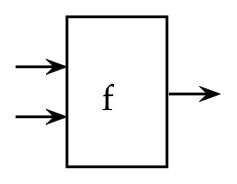
\includegraphics[width=1in]{notes/figs/n11/01oracle1.png}
        \caption{two-input Boolean function}
        \label{fig:01oracle1}
    \end{figure}
    
    We are told that $f$ is either AND or OR. We are allowed to supply inputs to test. This is the "oracle" part. The problem: how many trials (input configurations) are needed to tell whether $f=$ AND or $f=$ OR? Clearly, a single trial or function evaluation is sufficient shown in Figure \ref{fig:02oracle2}.
    
      \begin{figure}
        \centering
        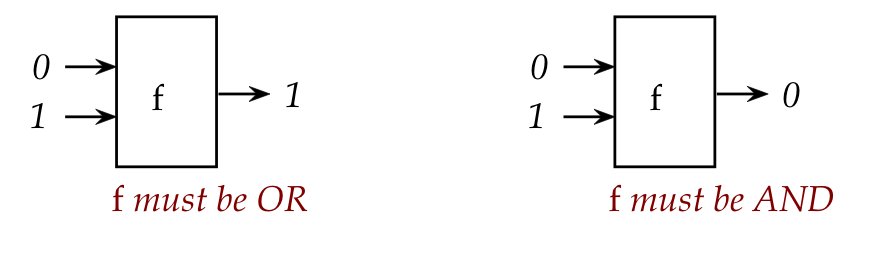
\includegraphics[width=4in]{notes/figs/n11/02oracle2.png}
        \caption{trials for $f=$ AND or $f=$ OR}
        \label{fig:02oracle2}
    \end{figure}
    
    But if we're told $f \in\{\mathrm{AND}, \mathrm{OR}, \mathrm{XOR}\}$, then a single evaluation is not sufficient as shown in Figure \ref{fig:03oracle3}.
    
    \begin{figure}
        \centering
        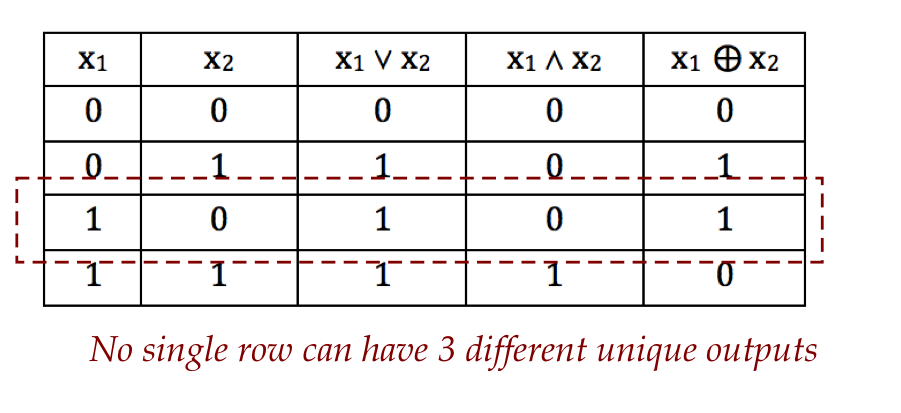
\includegraphics[width=4in]{notes/figs/n11/03oracle3.png}
        \caption{single evaluation not sufficient }
        \label{fig:03oracle3}
    \end{figure}
    
    Here, two evaluations suffice to determine which one. What is the quantum equivalent of an oracle problem? In this case, we will be given a unitary $U_{f}$ to which we can supply inputs shown in Figure \ref{fig:04oracle3b}.
    
    \begin{figure}
        \centering
        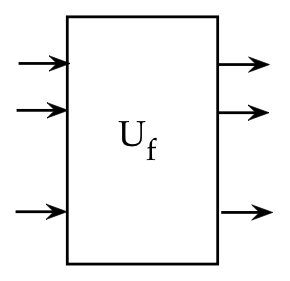
\includegraphics[width=4in]{notes/figs/n11/04oracle3b.png}
        \caption{Unitary $U_{f}$}
        \label{fig:04oracle3b}
    \end{figure}
    
    We are allowed to place circuitry before and after $U_{f}$, but $U_{f}$ itself is treated like an unknown blackbox shown in Figure \ref{fig:05oracle3c}.
    
    \begin{figure}
        \centering
        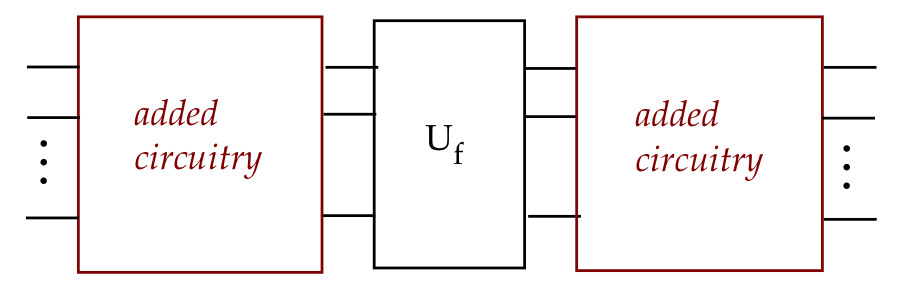
\includegraphics[width=4in]{notes/figs/n11/05oracle3c.png}
        \caption{Unknown Blackbox}
        \label{fig:05oracle3c}
    \end{figure}
    
    The question then is: how many trials are needed to decide whether a given $f$ has a certain property. In a quantum circuit, we are allowed ancillae, at the very least to compute $U_{f}$ shown in Figure \ref{fig:06oracle3d}.
    
    \begin{figure}
        \centering
        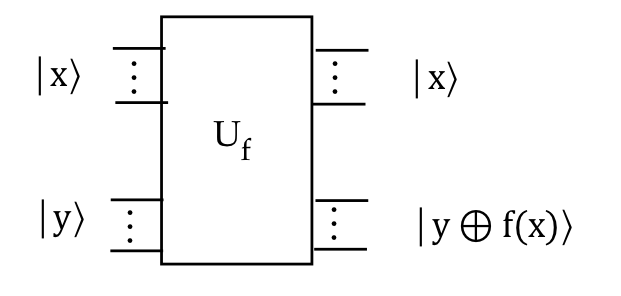
\includegraphics[width=4in]{notes/figs/n11/06oracle3d.png}
        \caption{Ancillae to compute $U_{f}$}
        \label{fig:06oracle3d}
    \end{figure}
    
    This is reasonable because we are going to focus on parallelism rather than the modest added cost of extra qubits. Such oracle problems are quite artificial but their impact has been significant: It at least shows cases where quantum algorithms are exponentially faster. The techniques used in the algorithms can be analyzed for application to practical problems. One such problem, Simon's problem, inspired a very practical breakthrough: Shor's integer factoring algorithm.

\subsection{Deutsch's algorithm}

    Deutsch's problem tries to boil down the quantum-classical difference to a single bit: There are only four possible single-bit functions shown in Figure \ref{fig:07oracle4}.
    
    \begin{figure}
        \centering
        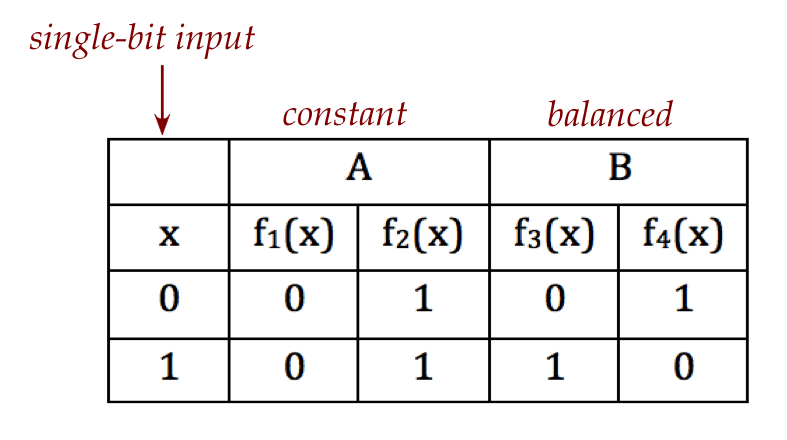
\includegraphics[width=4in]{notes/figs/n11/07oracle4.png}
            \caption{single-bit functions}
        \label{fig:07oracle4}
    \end{figure}
    
    The goal is to determine whether a mystery function $f$ is either in category A (that is, $f_{1}$ or $f_{2}$ ) or in category $\mathrm{B}\left(f_{3}\right.$ or $f_{4}$ ). Two trials are needed for a classical solution. What we will see is that superposition will let us solve the problem with a single trial with a quantum circuit. What is the quantum equivalent? We are given $U_{f}$ where $f$ is either in category A (constant) or category B (balanced) shown in Figure \ref{fig:08deutsch2}.
    
    \begin{figure}
        \centering
        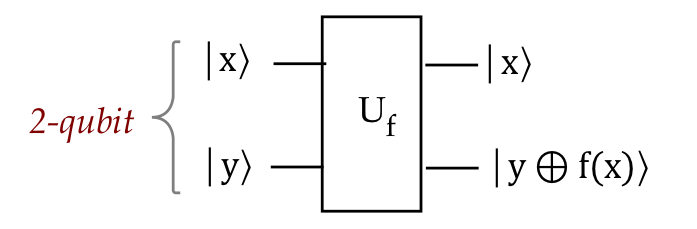
\includegraphics[width=4in]{notes/figs/n11/08deutsch2.png}
            \caption{Single-bit functions}
        \label{fig:08deutsch2}
    \end{figure}
    
    By evaluating (supplying inputs), we want to determine which category. For example, if $f(x)=0$ for both $x=0, x=1$, and we chose $|0\rangle$ as the ancilla, then outputs would be shown in Figure \ref{fig:09deutsch3}.
    
    \begin{figure}
        \centering
        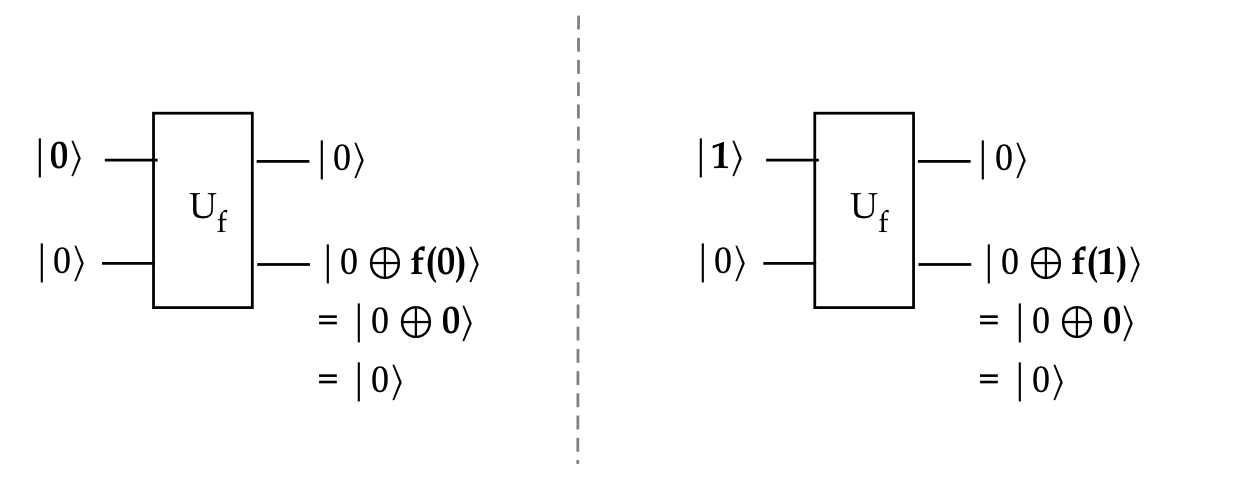
\includegraphics[width=4in]{notes/figs/n11/09deutsch3.png}
            \caption{Outputs}
        \label{fig:09deutsch3}
    \end{figure}
    
    Thus, our goal is to choose both input and ancilla carefully to minimize the number of trials. To begin, let's recall a consequence of global vs. relative phase: Suppose $x$ represents a single-bit Boolean value. Consider the two-qubit state
    
    $$
    |0\rangle \otimes|x\rangle+|1\rangle \otimes(-|x\rangle)
    $$
    
    Then
    
    $$
    \begin{aligned}
    |0\rangle \otimes|x\rangle+|1\rangle \otimes(-|x\rangle) &=|0\rangle \otimes|x\rangle+|1\rangle \otimes(-1)|x\rangle & &-1 \text { is a constant } \\
    &=|0\rangle \otimes|x\rangle+(-1)(|1\rangle \otimes|x\rangle) & & \text { Bilinearity } \\
    &=(|0\rangle+(-1)|1\rangle) \otimes|x\rangle & & \text { Tensor factoring } \\
    &=(|0\rangle-|1\rangle) \otimes|x\rangle & & \text { Simplification } \\
    &=\sqrt{2}|-\rangle \otimes|x\rangle & & \text { Recall }|-\rangle
    \end{aligned}
    $$
    
    On the other hand, consider the state
    $$
    |0\rangle \otimes(-|x\rangle)+|1\rangle \otimes(-|x\rangle)
    $$
    
    This simplifies as
    
    $$
    \begin{array}{rlr}
    |0\rangle \otimes(-|x\rangle)+|1\rangle \otimes(-|x\rangle) & =|0\rangle \otimes(-1)|x\rangle+|1\rangle \otimes(-1)|x\rangle & -1 \text { is a constant } \\
    & =(-1)(|0\rangle \otimes|x\rangle+|1\rangle \otimes|x\rangle) & \text { Bilinearity } \\
    & =e^{i \pi}(|0\rangle \otimes|x\rangle+|1\rangle \otimes|x\rangle) & \text { Emphasizing phase } \\
    & =(|0\rangle \otimes|x\rangle+|1\rangle \otimes|x\rangle) & \\
    & =(|0\rangle+|1\rangle) \otimes|x\rangle & \text { Global-phase equivalence } \\
    & =\sqrt{2}|+\rangle \otimes|x\rangle & \text { Tensor factoring }
    \end{array}
    $$
    
    Let's focus on the difference between the two starting states:
    
    $$
    \begin{aligned}
    (|0\rangle \otimes|x\rangle)+(|1\rangle \otimes(-|x\rangle)) &=(|0\rangle \otimes|x\rangle)-(|1\rangle \otimes|x\rangle)) \quad \text { Two terms have different sign } \\
    (|0\rangle \otimes(-|x\rangle))+(|1\rangle \otimes(-|x\rangle)) &=(|0\rangle \otimes|x\rangle)+(|1\rangle \otimes|x\rangle)) \quad \text { Two terms have same sign }
    \end{aligned}
    $$
    
    The same-vs-different sign works the same when
    
    $$
    \begin{aligned}
    (|0\rangle \otimes(-|x\rangle))+(|1\rangle \otimes|x\rangle)) &=(-1)(|0\rangle \otimes|x\rangle-|1\rangle \otimes|x\rangle)) \quad \text { Two terms have different sign, global-phase - 1 } \\
    (|0\rangle \otimes(|x\rangle))+(|1\rangle \otimes(|x\rangle)) &=(|0\rangle \otimes|x\rangle)+(|1\rangle \otimes|x\rangle))  \quad \text {Two terms have same sign} \\
    \end{aligned}
    $$
    
    In the first case we get $|-\rangle$ as the first qubit, and in the second, we get $|+\rangle$. We will exploit this difference now. We'll now apply $|+\rangle|-\rangle$ as input to $U_{f}$ : First, we'll expand $|+\rangle|-\rangle$ as
    
    $$
    \begin{aligned}
    |+\rangle|-\rangle &=\frac{1}{\sqrt{2}}(|0\rangle+|1\rangle)+\frac{1}{\sqrt{2}}(|0\rangle-|1\rangle) \\
    &=\frac{1}{2}(|0\rangle|0\rangle-|0\rangle|1\rangle+|1\rangle|0\rangle-|1\rangle|1\rangle)
    \end{aligned}
    $$
    
    Now
    
    $$
    U_{f}|x\rangle|y\rangle=|x\rangle|y \oplus f(x)\rangle
    $$
    
    for any $U_{f}$. Thus,
    
    $$
    \begin{aligned}
    U_{f}|+\rangle|-\rangle &=U_{f} \frac{1}{2}(|0\rangle|0\rangle-|0\rangle|1\rangle+|1\rangle|0\rangle-|1\rangle|1\rangle) \\
    &=\frac{1}{2}\left(U_{f}|0\rangle|0\rangle-U_{f}|0\rangle|1\rangle+U_{f}|1\rangle|0\rangle-U_{f}|1\rangle|1\rangle\right) \\
    &=\frac{1}{2}(|0\rangle|0 \oplus f(0)\rangle-|0\rangle|1 \oplus f(0)\rangle+|1\rangle|0 \oplus f(1)\rangle-|1\rangle|1 \oplus f(1)\rangle)
    \end{aligned}
    $$
    
    Consider the case when $f(x)=f_{1}(x)=0$ for both $x=0, x=1$: Then,
    
    $$
    \begin{aligned}
    U_{f}|+\rangle|-\rangle &=\frac{1}{2}(|0\rangle|0 \oplus 0\rangle-|0\rangle|1 \oplus 0\rangle+|1\rangle|0 \oplus 0\rangle\\
    &=\frac{1}{2}(|0\rangle|0\rangle-|0\rangle|1\rangle+|1\rangle|0\rangle-|1\rangle|1\rangle) \\
    &=\frac{1}{2}(|0\rangle(|0\rangle-|1\rangle)+|1\rangle(|0\rangle-|1\rangle)) \\
    &=\frac{1}{\sqrt{2}}(|0\rangle|-\rangle+|1\rangle|-\rangle) \\
    &=\frac{1}{\sqrt{2}}(|0\rangle+|1\rangle)|-\rangle \\
    &=|+\rangle|-\rangle
    \end{aligned}
    $$
    
    When $f(x)=f_{2}(x)=1$ for both $x=0, x=1$ we get the same result up to global phase:
    
    $$
    U_{f}|+\rangle|-\rangle=|+\rangle|-\rangle
    $$
    
    In-Class Exercise 2: Show that this is true. That is $U_{f_{2}}|+\rangle|-\rangle=|+\rangle|-\rangle$. Next, consider $f=f_{3}$ : In this case, $f_{3}(0)=0, f_{3}(1)=1$. Thus, with $f=f_{3}$ :
    
    $$
    \begin{aligned}
    U_{f}|+\rangle|-\rangle &=\frac{1}{2}(|0\rangle|0 \oplus f(0)\rangle-|0\rangle|1 \oplus f(0)\rangle+|1\rangle|0 \oplus f(1)\rangle-|1\rangle|1 \oplus f(1)\rangle) \\
    &=\frac{1}{2}(|0\rangle|0 \oplus 0\rangle-|0\rangle|1 \oplus 0\rangle+|1\rangle|0 \oplus 1\rangle-|1\rangle|1 \oplus 1\rangle) \\
    &=\frac{1}{2}(|0\rangle|0\rangle-|0\rangle|1\rangle+|1\rangle|1\rangle-|1\rangle|0\rangle) \\
    &=\frac{1}{2}(|0\rangle|0\rangle-|0\rangle|1\rangle+(-1)|1\rangle|0\rangle-(-1)|1\rangle|1\rangle) \\
    &=\frac{1}{2}(|0\rangle(|0\rangle-|1\rangle)-|1\rangle(|0\rangle-|1\rangle)) \\
    &=\frac{1}{\sqrt{2}}(|0\rangle-|1\rangle) \frac{1}{\sqrt{2}}(|0\rangle-|1\rangle) \\
    &=|-\rangle|-\rangle
    \end{aligned}
    $$
    
    Finally, when $f=f_{4}$, we get the same output with global phase:
    
    $$
    U_{f}|+\rangle|-\rangle=|-\rangle|-\rangle
    $$
    
    To summarize: When $f \in A$
    
    $$
    U_{f}|+\rangle|-\rangle=|+\rangle|-\rangle
    $$
    
    and when $f \in B$
    
    $$
    U_{f}|+\rangle|-\rangle=|-\rangle|-\rangle
    $$
    
    Thus if we measure the first qubit in H-basis, any $f \in A$ will always result in $|+\rangle$ output. And any $f \in B$ will result in $|-\rangle$ output. And, so with a single input and measurement, we can solve the problem. This demonstrates, for at least this oracle problem, that a quantum approach is demonstrably faster than classical. We can describe this visually in Figure \ref{fig:10deutsch4}.
    
    \begin{figure}
        \centering
        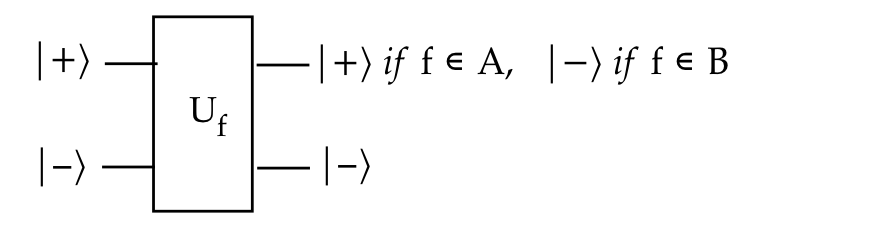
\includegraphics[width=5in]{notes/figs/n11/10deutsch4.png}
            \caption{single input solved problem}
        \label{fig:10deutsch4}
    \end{figure}
    
    Or fleshed out with measurement in \ref{fig:11deutsch5}.
    
    \begin{figure}
        \centering
        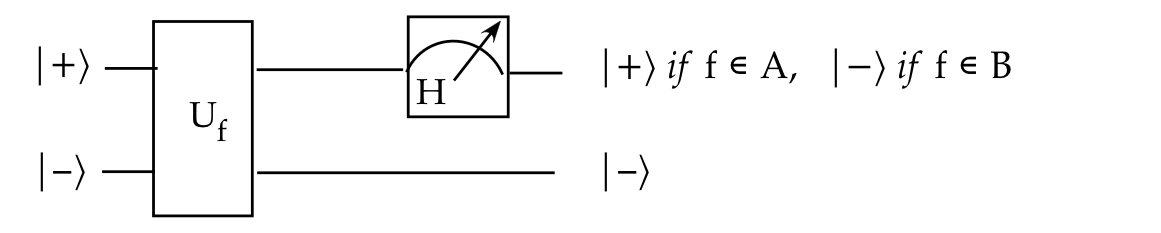
\includegraphics[width=5in]{notes/figs/n11/11deutsch5.png}
            \caption{fleshed out}
        \label{fig:11deutsch5}
    \end{figure}
    
    And using standard gates in Figure \ref{fig:12deutsch6}.
    
    \begin{figure}
        \centering
        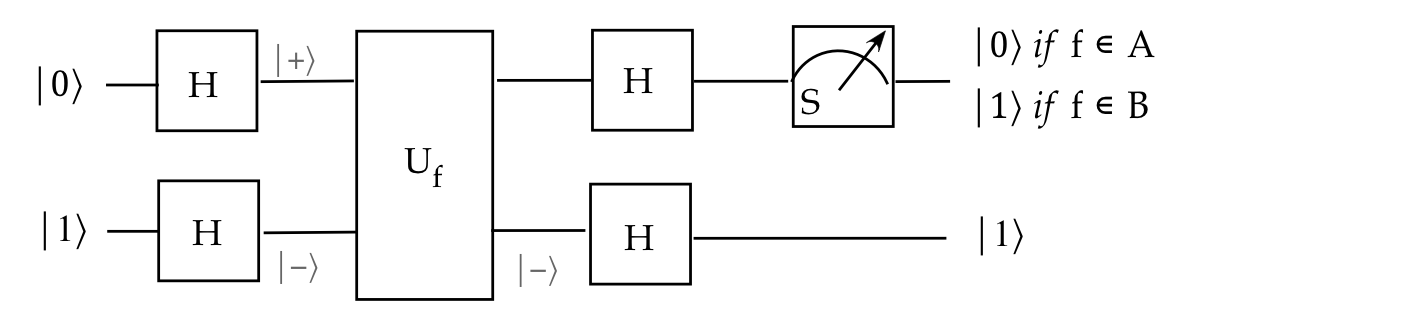
\includegraphics[width=5in]{notes/figs/n11/12deutsch6.png}
            \caption{Standard gates}
        \label{fig:12deutsch6}
    \end{figure}
    
    The doubling of speed for the single-bit problem above is not impressive. However, the same idea can be extended to demonstrate exponential speed up. But before getting to those examples, we'll need a few useful results.

\subsection{Some useful results}

    First, a result about the dot product of classical binary-vectors: As an example: the dot product of $x=(1,0,1)$ and $y=(1,1,0)$ is
    
    $$
    x \cdot y=(1,0,1) \cdot(1,1,0)=1
    $$
    
    and
    
    $$
    (1,0,1,1,1) \cdot(1,1,0,1,1)=3
    $$
    
    In general, for n-bit binary vectors:
    
    $$
    x \cdot y=\text { number of shared } 1 \text { s }
    $$
    
    Now, we'll use our shorthand notation to denote the binary vector $(1,0,1)$ by 101 or its decimal version 5: That is,
    
    $$
    (1,0,1)=101=5
    $$
    
    Then, all possible n-binary vectors can be written either as
    
    $$
    S=\{00 \ldots 0, \ldots,, 11 \ldots 1\}
    $$
    
    Or
    
    $$
    S=\left\{0, \ldots, 2^{n}-1\right\}
    $$
    
    We'll often use $N=2^{n}$. Proposition 10.1: Given an $n$-bit binary vector $y$,
    
    $$
    \sum_{x=0}^{N-1}(-1)^{x \cdot y}=\left\{\begin{array}{cc}
    N & \text { if } y=\mathbf{0} \\
    0 & \text { otherwise }
    \end{array}\right.
    $$
    
    Proof: Clearly, the case $y=0$ is obvious. Now suppose $y$ has $k 1^{\prime} s$ as in this example with $k=3$ shown in Figure \ref{13binaryvec}.
    
    \begin{figure}
        \centering
        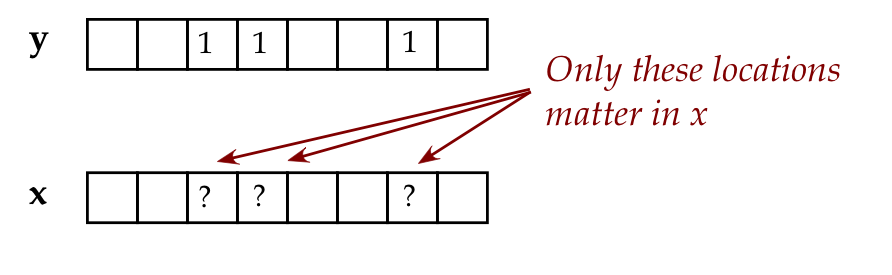
\includegraphics[width=4in]{notes/figs/n11/13binaryvec.png}
            \caption{$n$-bit binary vector $y$}
        \label{fig:13binaryvec}
    \end{figure}
    
    Since the summation cycles through all possible $x$, all possible $2^{k}$ bit-patterns will appear in the same locations where $y$ has 1's. Half of these will have an even number of 1's, the other half will have an odd number of 1's, as in this example with $k=3$ shown in Figure \ref{fig:14binaryvec2}.
    
    \begin{figure}
        \centering
        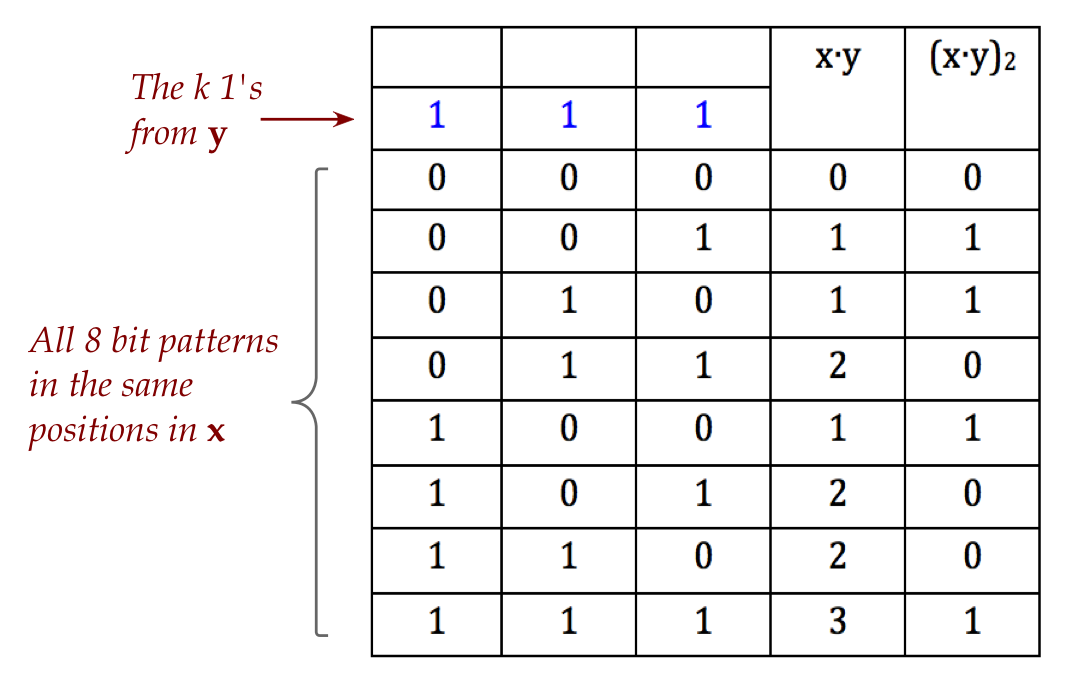
\includegraphics[width=4in]{notes/figs/n11/14binaryvec2.png}
            \caption{example with $k=3$}
        \label{fig:14binaryvec2}
    \end{figure}
    
    Thus, the $x \cdot y$ will be even for half of these patterns, and odd the rest. Then, $(-1)^{x \cdot y}=1$ for half, and $(-1)^{x \cdot y}=-1$ for the others. They thus cancel out. There is a variation of the dot-product that is also useful: We can define a mod-2 dot-product as
    
    $$
    (x \cdot y)_{2}=(x \cdot y) \bmod 2
    $$
    
    By examining the last column in the above table, we see that the same result in Proposition $10.1$ holds for this variation:
    
    $$
    \sum_{x=0}^{N-1}(-1)^{(x \cdot y)_{2}}=\left\{\begin{array}{cc}
    N & \text { if } y=0 \\
    0 & \text { otherwise }
    \end{array}\right.
    $$
    
    Next, let's review tensored Hadamards: Recall:
    
    $$
    \begin{aligned}
    &H|0\rangle=|+\rangle=\frac{1}{\sqrt{2}}(|0\rangle+|1\rangle) \\
    &H|1\rangle=|-\rangle=\frac{1}{\sqrt{2}}(|0\rangle-|1\rangle)
    \end{aligned}
    $$
    
    We can write this as
    
    $$
    H|x\rangle=\frac{1}{\sqrt{2}}\left(|0\rangle+(-1)^{x}|1\rangle\right)
    $$
    
    where $x$ is the binary variable $x \in\{0,1\}$. We'll take this a step further by introducing a second variable $y$ :
    
    $$
    \begin{aligned}
    H|x\rangle &=\frac{1}{\sqrt{2}}\left(|0\rangle+(-1)^{x}|1\rangle\right) \\
    &=\frac{1}{\sqrt{2}}\left((-1)^{0}|y=0\rangle+(-1)^{x}|y=1\rangle\right) \\
    &=\frac{1}{\sqrt{2}}\left((-1)^{0 \cdot y}|y=0\rangle+(-1)^{x \cdot y}|y=1\rangle\right) \\
    &=\frac{1}{\sqrt{2}} \sum_{y=0}^{1}(-1)^{x y}|y\rangle
    \end{aligned}
    $$
    
    Now recall that $H^{\otimes n}$ applied to $|00 \ldots 0\rangle$ produces the equal superposition:
    
    $$
    H^{\otimes n}|00 \ldots 0\rangle=\frac{1}{\sqrt{N}} \sum_{y}^{N-1}|y\rangle
    $$
    
    where $N=2^{n}$ and $y$ is in decimal form:
    
    $$
    |y\rangle \in\{|0\rangle,|1\rangle,|2\rangle, \ldots,|N-1\rangle\}
    $$
    
    We'll use our new notation to derive this easily:
    
    $$
    \begin{aligned}
    H^{\otimes n}|00 \ldots 0\rangle &=(H \otimes H \otimes \ldots \otimes H)|0\rangle|0\rangle \ldots|0\rangle \\
    &=H|0\rangle \otimes H|0\rangle \otimes \ldots \otimes H|0\rangle \\
    &=\left(\frac{1}{\sqrt{2}} \sum_{y_{n-1}=0}^{1}\left|y_{n-1}\right\rangle\right) \otimes\left(\frac{1}{\sqrt{2}} \sum_{y_{n-2}=0}^{1}\left|y_{n-2}\right\rangle\right) \otimes \ldots \otimes\left(\frac{1}{\sqrt{2}} \sum_{y_{0}=0}^{1}\left|y_{0}\right\rangle\right) \\
    &=\frac{1}{\sqrt{N}} \sum_{y_{n-1}, \ldots, y_{0}}\left|y_{n-1}\right\rangle\left|y_{n-2}\right\rangle \ldots\left|y_{0}\right\rangle \\
    &=\frac{1}{\sqrt{N}} \sum_{y=0}^{N-1}|y\rangle
    \end{aligned}
    $$
    
    where we switched to decimal in the last step. Note: we have applied $H^{\otimes n}$ to the standard-basis vector $|00 \ldots 0\rangle$. We are going to need to see what we get when $H^{\otimes n}$ is applied to any other standard basis vector. Conveniently, it has a compact form:
    Proposition 10.2:
    
    $$
    H^{\otimes n}|x\rangle=\frac{1}{\sqrt{N}} \sum_{y=0}^{N-1}(-1)^{x \cdot y}|y\rangle
    $$
    
    Proof:
    
    $$
    \begin{aligned}
    H^{\otimes n}|x\rangle &=(H \otimes H \otimes \ldots \otimes H)\left|x_{n-1}\right\rangle\left|x_{n-1}\right\rangle \ldots\left|x_{0}\right\rangle \\
    &=H\left|x_{n-1}\right\rangle \otimes\left|x_{n-1}\right\rangle \otimes \ldots \otimes H\left|x_{0}\right\rangle \\
    &=\left(\frac{1}{\sqrt{2}} \sum_{y_{n-1}=0}^{1}(-1)^{x_{n-1} y_{n-1}}\left|y_{n-1}\right\rangle\right) \otimes\left(\frac{1}{\sqrt{2}} \sum_{y_{n-2}=0}^{1}(-1)^{x_{n-2} y_{n-2}}\left|y_{n-2}\right\rangle\right) \otimes \ldots \otimes\left(\frac{1}{\sqrt{2}} \sum_{y_{0}=0}^{1}(-1)^{x_{0} y_{0}}\left|y_{0}\right\rangle\right) \\
    &=\frac{1}{\sqrt{N}} \sum_{y_{n-1}, \ldots, y_{0}}(-1)^{x_{n-1} y_{n-1}}(-1)^{x_{n-2} y_{n-2}} \ldots(-1)^{x_{0} y_{0}}\left|y_{n-1}\right\rangle\left|y_{n-2}\right\rangle \ldots\left|y_{0}\right\rangle \\
    &=\frac{1}{\sqrt{N}} \sum_{y=0}^{N-1}(-1)^{x_{n-1} y_{n-1}+x_{n-2} y_{n-2} \ldots x_{0} y_{0}}|y\rangle \\
    &=\frac{1}{\sqrt{N}} \sum_{y=0}^{N-1}(-1)^{x \cdot y}|y\rangle
    \end{aligned}
    $$

\subsection{The Deutsch-Jozsa algorithm}

    Let's first state the problem: Let $S_{n}=2^{\{0,1\}}=$ all n-bit binary patterns. Here, we consider Boolean functions $f: S_{n} \rightarrow\{0,1\}$. That is, n-bit input, and 1-bit output. A function $f$ is constant if either: 1. $f(x)=0$ for all $x$ and 2. $f(x)=1$ for all $x$. A function $f$ is balanced if $f(x)=0$ for exactly half the inputs $x \in S_{n}$. That is,
    
    $$
    |\{x: f(x)=0\}|=\frac{2^{n}}{2}
    $$
    
    The objective of the problem: We are given that $f$ is either constant or balanced. How many trials (different evaluations with inputs) does it take to distinguish whether constant or balanced? The classical solution will, in the worst-case, need to evaluate just over half the inputs $2^{n-1}+1$ trials. We will show that a single trial is sufficient for a quantum algorithm. An exponential speed up.
    To begin, let's take a closer look at the output qubit in our customary set up: First, we'll use the symmetry of XOR to write $|f(x) \oplus y\rangle$ shown in Figure \ref{fig:15deutsch7}.
    
    \begin{figure}
        \centering
        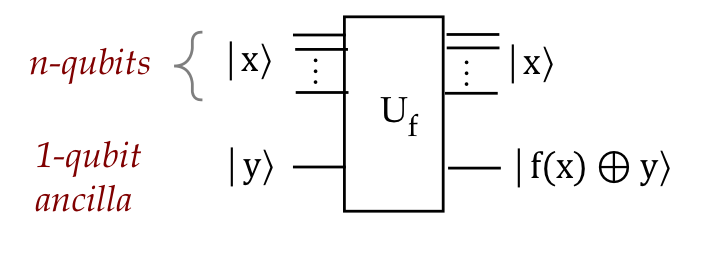
\includegraphics[width=4in]{notes/figs/n11/15deutsch7.png}
            \caption{$|f(x) \oplus y\rangle$}
        \label{fig:15deutsch7}
    \end{figure}
    
    Here, $y \in\{0,1\}$ is a single bit. Notice: When $f(x)=0$, the output is just $y$. When $f(x)=1$, the output is $y^{\prime}$. That is, $f(x)=1$ "flips" $y$. We can think of this as applying the $X$ gate to $|y\rangle$ whenever it is controlled by $f(x)$. Now let's ask: what if $|y\rangle$ were any qubit state? Let $|y\rangle=\alpha|0\rangle+\beta|1\rangle$. Consider $f(x)=0$. Then,
    
    $$
    \begin{aligned}
    U_{f}|x\rangle|y\rangle &=U_{f}|x\rangle(\alpha|0\rangle+\beta|1\rangle) \\
    &=\alpha U_{f}|x\rangle|0\rangle+\beta U_{f}|x\rangle|1\rangle \\
    &=\alpha|x\rangle|f(x) \oplus 0\rangle+\beta|x\rangle|f(x) \oplus 1\rangle \\
    &=\alpha|x\rangle|0 \oplus 0\rangle+\beta|x\rangle|0 \oplus 1\rangle \\
    &=\alpha|x\rangle|0\rangle+\beta|x\rangle|1\rangle \\
    &=|x\rangle(\alpha|0\rangle+\beta|1\rangle) \\
    &=|x\rangle|y\rangle
    \end{aligned}
    $$
    
    And when $f(x)=1$
    
    $$
    \begin{aligned}
    U_{f}|x\rangle|y\rangle &=\alpha|x\rangle|f(x) \oplus 0\rangle+\beta|x\rangle|f(x) \oplus 1\rangle \\
    &=\alpha|x\rangle|1 \oplus 0\rangle+\beta|x\rangle|1 \oplus 1\rangle \\
    &=\alpha|x\rangle|1\rangle+\beta|x\rangle|0\rangle \\
    &=|x\rangle(\alpha|1\rangle+\beta|0\rangle) \\
    &=|x\rangle(X|y\rangle)
    \end{aligned}
    $$
    
    Thus, it does work for arbitrary $|y\rangle$. Now consider the special case $|y\rangle=|-\rangle$: When $f(x)=0$ :
    
    $$
    U_{f}|x\rangle|-\rangle=|x\rangle|-\rangle
    $$
    
    When $f(x)=1$ :
    
    $$
    U_{f}|x\rangle|-\rangle=|x\rangle X|-\rangle=|x\rangle(-1)|-\rangle
    $$
    
    because $X|-\rangle=-|-\rangle$. We can summarize this as:
    
    $$
    U_{f}|x\rangle|-\rangle=(-1)^{f(x)}|x\rangle|-\rangle
    $$
    
    Now we can see what $U_{f}$ does to the equal superposition:
    Proposition 10.3:
    
    $$
    U_{f} \frac{1}{\sqrt{N}} \sum_{x}|x\rangle|-\rangle=\frac{1}{\sqrt{N}} \sum_{x}(-1)^{f(x)}|x\rangle|-\rangle
    $$
    
    Proof: Simple application of the linearity of $U_{f}$. Now to the algorithm: Let
    
    $$
    |\psi\rangle=U_{f} \frac{1}{\sqrt{N}} \sum_{x}|x\rangle|-\rangle=\frac{1}{\sqrt{N}} \sum_{x}(-1)^{f(x)}|x\rangle|-\rangle
    $$
    
    That is shown in Figure \ref{fig:16deutsch8}.
    
    \begin{figure}
        \centering
        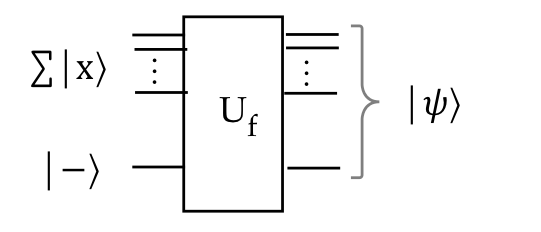
\includegraphics[width=3in]{notes/figs/n11/16deutsch8.png}
            \caption{$U_{f}$}
        \label{fig:16deutsch8}
    \end{figure}
    
    Now apply $H^{\otimes n} \otimes I$ to this shown in Figure \ref{fig:17deutsch9}.
    
    \begin{figure}
        \centering
        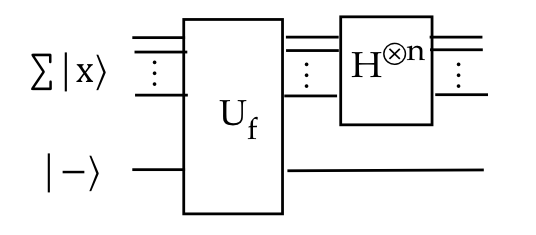
\includegraphics[width=3in]{notes/figs/n11/17deutsch9.png}
            \caption{apply $H^{\otimes n} \otimes I$}
        \label{fig:17deutsch9}
    \end{figure}
    
    $$
    \begin{aligned}
    \left(H^{\otimes n} \otimes I\right)|\psi\rangle &=\left(H^{\otimes n} \otimes I\right) \frac{1}{\sqrt{N}} \sum_{x}(-1)^{f(x)}|x\rangle|-\rangle \\
    &=\frac{1}{\sqrt{N}} \sum_{x}(-1)^{f(x)} H^{\otimes n}|x\rangle|-\rangle
    \end{aligned}
    $$
    
    Recall Proposition 10.2:
    
    $$
    H^{\otimes n}|x\rangle=\frac{1}{\sqrt{N}} \sum_{y=0}^{N-1}(-1)^{x \cdot y}|y\rangle
    $$
    
    Substituting above:
    
    $$
    \begin{aligned}
    \left(H^{\otimes n} \otimes I\right)|\psi\rangle &=\frac{1}{\sqrt{N}} \sum_{x}(-1)^{f(x)} \frac{1}{\sqrt{N}}\left(\sum_{y=0}^{N-1}(-1)^{x \cdot y}|y\rangle\right)|-\rangle \\
    &=\frac{1}{N} \sum_{x, y}(-1)^{f(x)}(-1)^{x \cdot y}|y\rangle|-\rangle
    \end{aligned}
    $$
    
    This looks to be an unwieldy expression, but let's separate out $|y\rangle=|0\rangle$ :
    
    $$
    \begin{aligned}
    \left(H^{\otimes n} \otimes I\right)|\psi\rangle &=\frac{1}{N} \sum_{x, y=0}(-1)^{f(x)}(-1)^{x \cdot y}|0\rangle|-\rangle+\frac{1}{N} \sum_{x, y \neq 0}(-1)^{f(x)}(-1)^{x \cdot y}|y\rangle|-\rangle \\
    &=\frac{1}{N}\left(\sum_{x, y=0}(-1)^{f(x)}\right)|0\rangle|-\rangle+\frac{1}{N} \sum_{x}(-1)^{f(x)}(-1)^{x \cdot y}|y\rangle|-\rangle
    \end{aligned}
    $$
    
    where $|0\rangle|-\rangle$ is factored out since neither depend on $x$. Now focus on the coefficient next to $|0\rangle|-\rangle$ :
    
    $$
    \frac{1}{N}\left(\sum_{x}(-1)^{f(x)}\right)=\frac{1}{N} \sum_{x}(-1)^{f(x)}
    $$
    
    If $f(x)=0$ for all $x$ :
    
    $$
    \frac{1}{N} \sum_{x=0}^{N-1}(-1)^{f(x)}=1
    $$
    
    And if $f(x)=1$ for all $x$ :
    
    $$
    \frac{1}{N} \sum_{x=0}^{N-1}(-1)^{f(x)}=-1
    $$
    
    Thus, if $f$ is constant, the squared coefficient is 1 . If $f(x)$ is balanced, then from Proposition 10.1,
    
    $$
    \sum_{x=0}^{N-1}(-1)^{f(x)}=0
    $$
    
    and so the coefficient of $|0\rangle|-\rangle$ is 0. To summarize: If $f$ is constant, the coefficient of $|0\rangle|-\rangle$ is 1. If $f$ is balanced, the coefficient of $|0\rangle|-\rangle$ is 0. Thus, a single measurement of the top $n$ qubits in the S-basis will clearly distinguish the two types: If the outcome is $|0\rangle, f$ is constant. If the outcome is any other vector, $f$ is balanced. We can now add the other pieces to complete the circuit shown in Figure \ref{fig:18deutsch10}.
    
    
    \begin{figure}
        \centering
        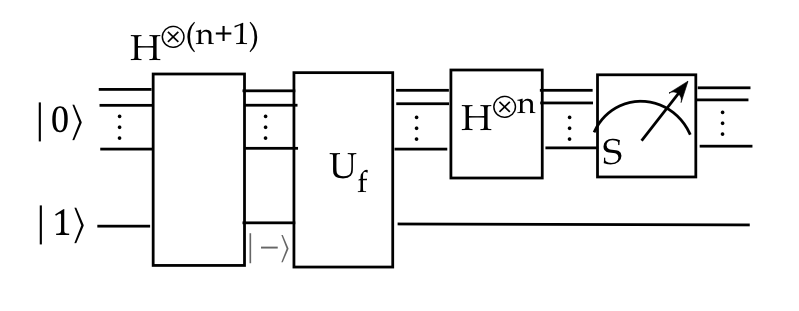
\includegraphics[width=4in]{notes/figs/n11/18deutsch10.png}
            \caption{complete circuit}
        \label{fig:18deutsch10}
    \end{figure}
    
    What do we learn from this example? We already know that $H^{\otimes n}$ is useful in producing the equal n-qubit superposition. But we now see that $H^{\otimes n}$ can be useful in the middle of a circuit as well. Using $|-\rangle$ as an ancilla value results in getting signs $(-1)^{f(x)}$ entangled with different states in the superposition: Then, by analyzing how the signs for a pattern, we saw how one state's amplitude was boosted. We got lucky that the boost was maximal (probability = 1). Even if not maximal, we could repeat the entire process so that a high-probability informative state is measured as outcome. One new trick learned: We don't need to fully analyze a complicated expression. Just knowing a key state's amplitude was boosted might be enough. We also need to acknowledge: this is a highly artificial problem, almost designed in reverse.

\subsection{The Bernstein-Vazirani algorithm}

    First, the problem: In the following, we'll assume the dot-operator in applies with mod-2:
    
    $$
    (c \cdot x)_{2}=\left(\sum_{i} c_{i} x_{i}\right) \bmod 2
    $$
    
    An alternate notation is:
    
    $$
    (c \cdot x)_{2}={ }_{2} \quad c \cdot x
    $$
    
    Let $f(x)=(c \cdot x)_{2}$ be a Boolean function where both $c$ and $x$ are binary strings or vectors. We are given a blackbox that implements $f(x) \bmod 2$ but not told what $c$ is. The goal is to find $c$ using a minimum number of queries. Note: the output $f(x) \bmod 2$ is a single bit. For example, suppose $c=101$. When using $x=100$, we see that $f(x)=(101) \cdot(100)=1$, from which we conclude the first bit of $c$ is 1 . Then, using $x=010$, the second bit is 0. And, using $x=001$, the third bit 1. Note: using $x=111$ is not useful because $f(x)=(101) \cdot(111)=0$. We can't conclude anything definitive. Thus, the classical approach requires $n$ queries. We'll now see that a quantum algorithm can return $c$ in a single query. The algorithm: The machinery of Deutsch-Jozsa can be used to solve this problem using $f(x)=(c \cdot x)_{2}$. We start the same way with
    
    $$
    |\psi\rangle=U_{f} \frac{1}{\sqrt{N}} \sum_{x}|x\rangle|-\rangle=\frac{1}{\sqrt{N}} \sum_{x}(-1)^{f(x)}|x\rangle|-\rangle
    $$
    
    and apply $H^{\otimes n} \otimes I$ to get
    
    $$
    \left(H^{\otimes n} \otimes I\right)|\psi\rangle \frac{1}{N} \sum_{x, y}(-1)^{f(x)}(-1)^{(x \cdot y)_{2}}|y\rangle|-\rangle
    $$
    
    At this point, we substitute for the new $f(x)$ in this problem:
    
    $$
    \left(H^{\otimes n} \otimes I\right)|\psi\rangle \frac{1}{N} \sum_{x, y}(-1)^{(c \cdot x)_{2}}(-1)^{(x \cdot y)_{2}}|y\rangle|-\rangle
    $$
    
    In Deutsch-Jozsa, we separated out the term with $|0\rangle|-\rangle$. Here, we'll examine the term $|c\rangle|-\rangle$. That is, when $y=c$. The coefficient of $|c\rangle|-\rangle$ is:
    
    $$
    \begin{aligned}
    \frac{1}{N} \sum_{x}(-1)^{(c \cdot x)_{2}}(-1)^{(c \cdot x)_{2}}|c\rangle|-\rangle &=\left(\frac{1}{N} \sum_{x}(-1)^{(c \cdot x)_{2}}(-1)^{(c \cdot x)_{2}}\right)|c\rangle|-\rangle \\
    &=\left(\frac{1}{N} \sum_{x}(1)\right)|c\rangle|-\rangle \\
    &=\left(\frac{1}{N} N\right)|c\rangle|-\rangle \\
    &=|c\rangle|-\rangle
    \end{aligned}
    $$
    
    That is, happily, $|c\rangle$ is the only outcome possible. Thus, the same circuit as in Deutsch-Jozsa with the new $f$ directly produces $c$ as its only outcome from a single measurement shown in Figure \ref{fig:19bernstein}.
    
    \begin{figure}
        \centering
        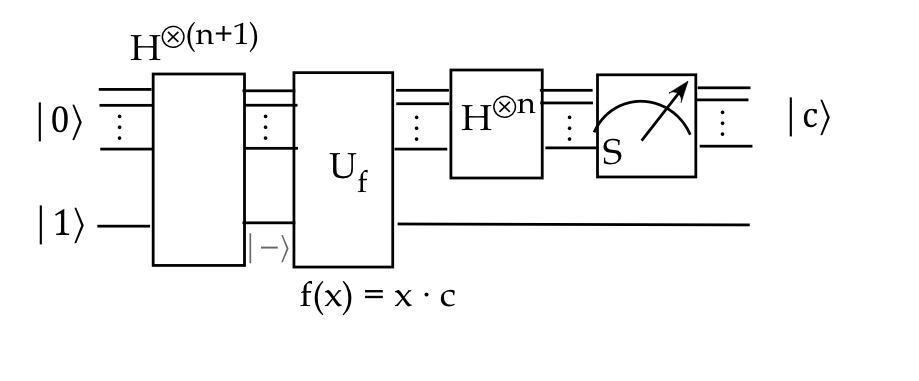
\includegraphics[width=4in]{notes/figs/n11/19bernstein.png}
            \caption{Same circuit as in Deutsch-Jozsa with the new $f$}
        \label{fig:19bernstein}
    \end{figure}

\subsection{Simon's algorithm}

    First, two tiny useful results: Proposition 10.4: For binary vectors $x, y, c$: 1. $x \oplus y=y \oplus x$, 2. $x \oplus(c \oplus y)=(x \oplus c) \oplus y$, 3. If $x \oplus c=y$ then: i. $x \oplus y=c$ ii. $y \oplus c=x$. Proof: The commutativity and associativity follow from examining each bit. Clearly, $x_{i} \oplus y_{i}=y_{i} \oplus x_{i}$ For associativity, we can write out the truth-table shown in Figure \ref{fig:20simon1}.
    
    \begin{figure}
        \centering
        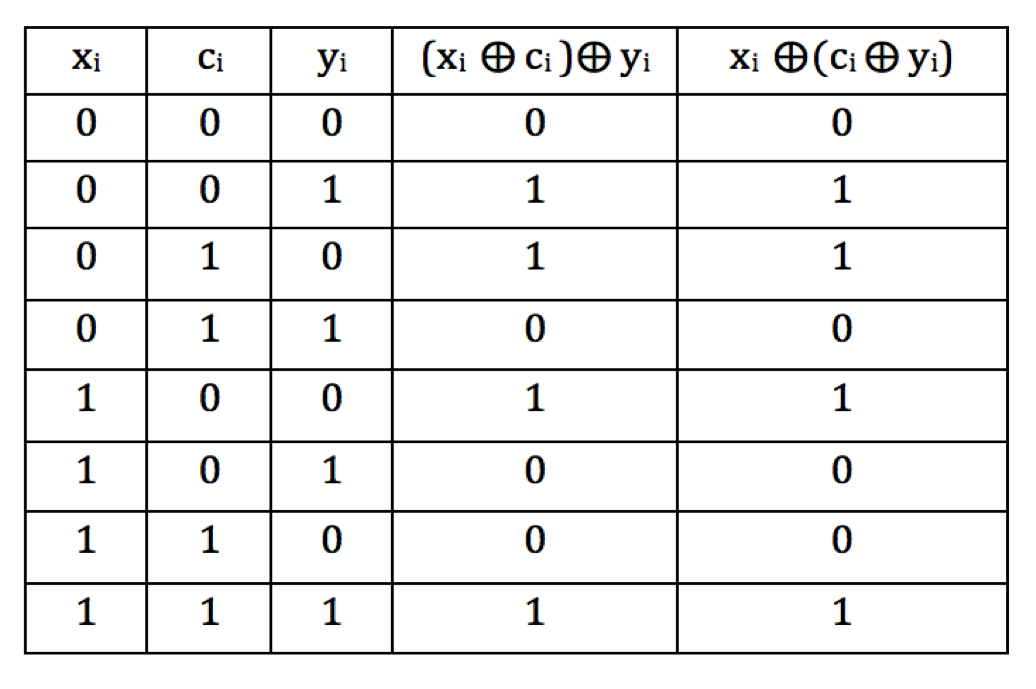
\includegraphics[width=4in]{notes/figs/n11/20simon1.png}
            \caption{Associativity truth-table}
        \label{fig:20simon1}
    \end{figure}
    
    Because no bit affects any other, the result holds for the vectors. From
    
    $$
    y=x \oplus c
    $$
    
    we get
    
    $$
    y \oplus c=(x \oplus c) \oplus c=x \oplus(c \oplus c)=x
    $$
    
    or
    
    $$
    y \oplus c=x
    $$
    
    Left-XORing this with $y$ gives us the second result. Proposition 10.5: For binary vectors $x, y, c$ :
    
    $$
    (x \oplus c) \cdot y=2 \quad x \cdot y+c \cdot y
    $$
    
    Proof: The proof follows by working out the truth table for single bits shown in Figure \ref{fig:21simon1b}.
    
    \begin{figure}
        \centering
        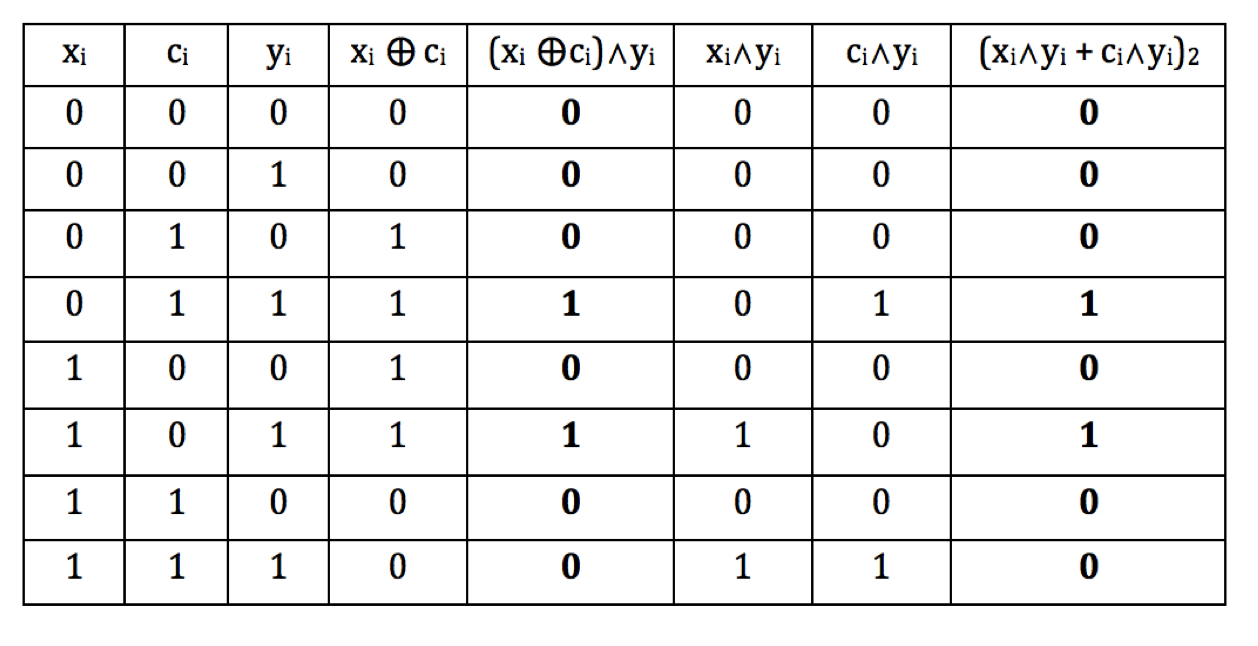
\includegraphics[width=5in]{notes/figs/n11/21simon1b.png}
            \caption{Truth table for single bits}
        \label{fig:21simon1b}
    \end{figure}
    
    Now let's describe the problem to be solved: We are given a function $f: S_{n} \rightarrow S_{n}$, that is, from n-bit strings to $\mathrm{n}$-bit strings. The function $f$ has the following two properties: 1. $f$ is 2-to-1: for any $x$, there is exactly one $y$ such that $f(x)=f(y)$. 2. There is an unknown vector $c$ such that $f(x \oplus c)=f(x)$ for all $x$. $\triangleright$ The goal: find $c$. Thus, when $f(x)=f(y)$, we are given that $y=c \oplus x$. Here's a 3-bit example with $c=110$ shown in Figure \ref{fig:22simon2}.
    
    \begin{figure}
        \centering
        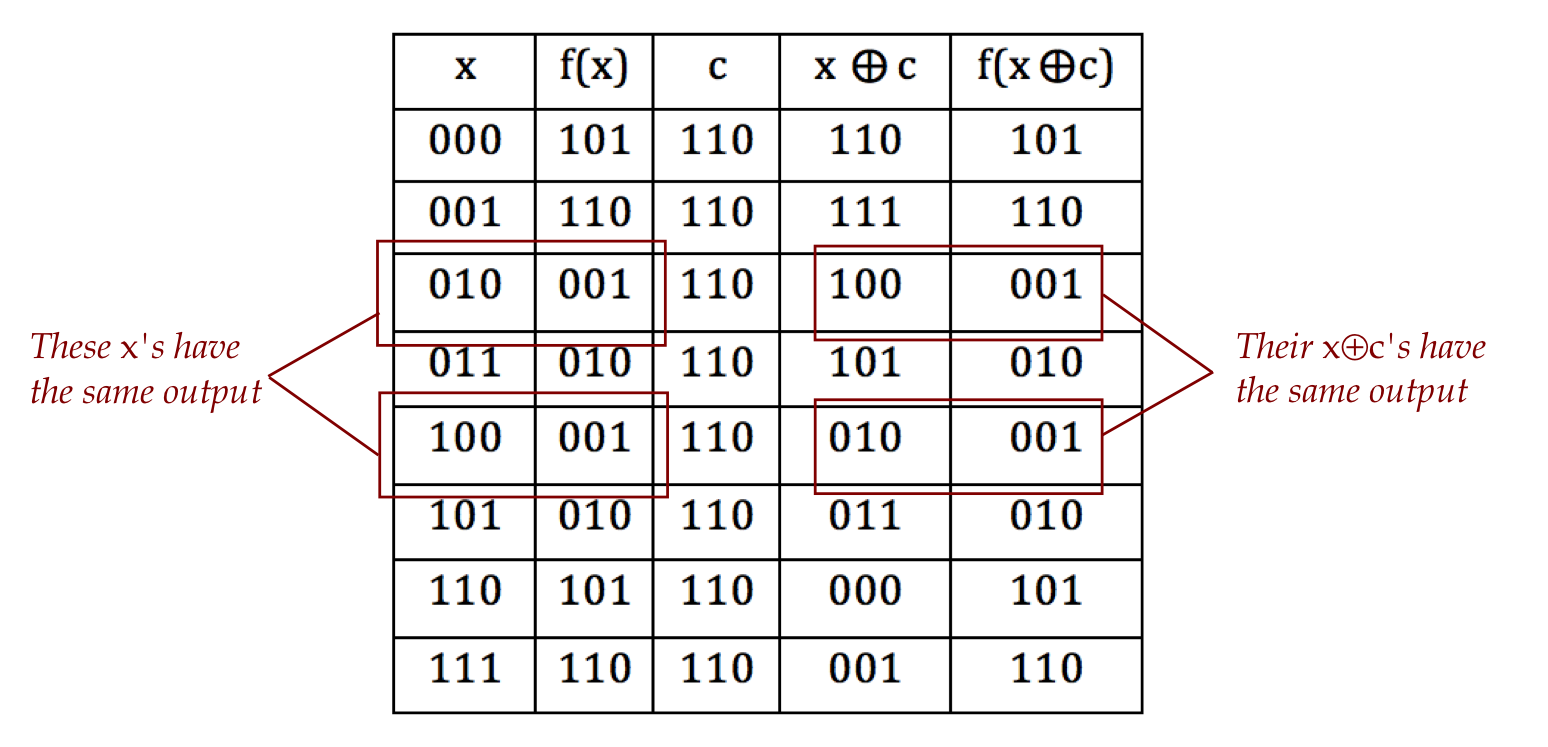
\includegraphics[width=5in]{notes/figs/n11/22simon2.png}
            \caption{3-bit example with $c=110$}
        \label{fig:22simon2}
    \end{figure}
    
    The number $c$ is something like a period: For a real function $f(x)$, if $f(x+T)=f(x)$, then $T$ is called the period. Because the condition $f(x \oplus c)=f(x)$ is similar, $c$ is called the period in this case. Note: there is no equivalent notion of distance in this binary case. The goal of the problem: discover the period $c$ with as few queries (function evaluations) as possible. How long does the best classical algorithm need? Such an algorithm needs to try $x$ and $y$ until the first such pair gives $f(x)=f(y)$. At this time, we know $x \oplus c=y$. From Proposition 10.4, we know then that $c=x \oplus y$. What is the best one can do in trying different $x$? Suppose we start at $x=0$, and try every $x$ in sequence: $x=1, x=2, \ldots$. Then we are guaranteed to find at least one repeat $f(x)$. $2^{n-1}+1$ evaluations worst-case. Simon's algorithm: The starting point is the full-superposition and an ancilla of $|00 \ldots 0\rangle$ :
    
    $$
    |\psi\rangle=\frac{1}{\sqrt{N}} \sum_{x}|x\rangle|0\rangle
    $$
    
    Now apply $U_{f}$ :
    
    $$
    \begin{aligned}
    U_{f}|\psi\rangle &=\frac{1}{\sqrt{N}} \sum_{x} U_{f}|x\rangle|0\rangle \\
    &=\frac{1}{\sqrt{N}} \sum_{x}|x\rangle|0 \oplus f(x)\rangle \\
    &=\frac{1}{\sqrt{N}} \sum_{x}|x\rangle|f(x)\rangle
    \end{aligned}
    $$
    
    Note: because $f: S_{n} \rightarrow S_{n}$, the vector $|f(x)\rangle$ is an n-qubit vector. Next, we measure this set of qubits (the second $n$ qubits) in the S-basis. Which means the outcome vector will be $\left|f\left(x^{\prime}\right)\right\rangle$ for some input bit pattern $x^{\prime}$. Now because there are two inputs that result in this output value, there is some $y^{\prime}$ such that
    
    $$
    \left|f\left(y^{\prime}\right)\right\rangle=\left|f\left(x^{\prime}\right)\right\rangle
    $$
    
    where
    
    $$
    y^{\prime}=x^{\prime} \oplus c
    $$
    
    Examine now the original $2 \mathrm{n}$-qubit output before measurement:
    
    $$
    U_{f}|\psi\rangle=\frac{1}{\sqrt{N}} \sum_{x}|x\rangle|f(x)\rangle
    $$
    
    Because $|x\rangle|f(x)\rangle$ are entangled, if measurement shows $\left|f\left(x^{\prime}\right)\right\rangle$, then the top $\mathrm{n}$-qubits will have some combination of $\left|x^{\prime}\right\rangle$ or $\left|y^{\prime}\right\rangle$. That is, the outcome will be a linear combination
    
    $$
    \text { (constant) }\left|x^{\prime}\right\rangle\left|f\left(x^{\prime}\right)\right\rangle+\text { (constant) }\left|y^{\prime}\right\rangle\left|f\left(y^{\prime}\right)\right\rangle
    $$
    
    But all the inputs are in equal superposition, so the outcome is in fact:
    
    $$
    \frac{1}{\sqrt{2}}\left|x^{\prime}\right\rangle\left|f\left(x^{\prime}\right)\right\rangle+\frac{1}{\sqrt{2}}\left|y^{\prime}\right\rangle\left|f\left(y^{\prime}\right)\right\rangle
    $$
    
    Which simplifies to:
    
    $$
    \frac{1}{\sqrt{2}}\left(\left|x^{\prime}\right\rangle+\left|y^{\prime}\right\rangle\right)\left|f\left(x^{\prime}\right)\right\rangle
    $$
    
    (Since $f\left(x^{\prime}\right)=f\left(y^{\prime}\right)$ ) Finally, substitute $y^{\prime}=x^{\prime} \oplus c$ to get:
    
    $$
    \frac{1}{\sqrt{2}}\left(\left|x^{\prime}\right\rangle+\left|x^{\prime} \oplus c\right\rangle\right)\left|f\left(x^{\prime}\right)\right\rangle
    $$
    
    Let's call this $\left|\psi_{2}\right\rangle$ :
    
    $$
    \left|\psi_{2}\right\rangle=\frac{1}{\sqrt{2}}\left(\left|x^{\prime}\right\rangle+\left|x^{\prime} \oplus c\right\rangle\right)\left|f\left(x^{\prime}\right)\right\rangle
    $$
    
    Recall the mod-2 variation of Proposition 10.2:
    
    $$
    H^{\otimes n}|x\rangle=\frac{1}{\sqrt{N}} \sum_{y}^{N-1}(-1)^{(x \cdot y)_{2}}|y\rangle
    $$
    
    We now apply $H^{\otimes n}$ to the top n qubits:
    
    $$
    \begin{aligned}
    \left(H^{\otimes n} \otimes I_{n}\right)\left|\psi_{2}\right\rangle &=\left(H^{\otimes n} \otimes I_{n}\right) \frac{1}{\sqrt{2}}\left(\left|x^{\prime}\right\rangle+\left|x^{\prime} \oplus c\right\rangle\right)\left|f\left(x^{\prime}\right)\right\rangle \\
    &=\frac{1}{\sqrt{2}} \frac{1}{\sqrt{N}} \sum_{y}\left((-1)^{\left(x^{\prime} \cdot y\right)_{2}}+(-1)^{\left(\left(x^{\prime} \oplus c\right) \cdot y\right)_{2}}\right)|y\rangle\left|f\left(x^{\prime}\right)\right\rangle \\
    &=\frac{1}{\sqrt{2}} \frac{1}{\sqrt{N}} \sum_{y}\left((-1)^{\left(x^{\prime} \cdot y\right)_{2}}+(-1)^{\left(x^{\prime} \cdot y\right)_{2}}(-1)^{(c \cdot y)_{2}}\right)|y\rangle\left|f\left(x^{\prime}\right)\right\rangle \\
    &=\frac{1}{\sqrt{2}} \frac{1}{\sqrt{N}} \sum_{y}\left((-1)^{\left(x^{\prime} \cdot y\right)_{2}}\left[1+(-1)^{(c \cdot y)_{2}}\right]\right)|y\rangle\left|f\left(x^{\prime}\right)\right\rangle
    \end{aligned}
    $$
    
    Note: in going to the third step, we applied Proposition 10.5. Now,
    
    $$
    \left[1+(-1)^{(c \cdot y)_{2}}\right]= \begin{cases}2 & \text { if } c \cdot y={ }_{2} 0 \\ 0 & \text { if } c \cdot y={ }_{2} 1\end{cases}
    $$
    
    Thus, any measurement of the top $\mathrm{n}$ qubits, will produce as outcome some $|y\rangle$ such $c \cdot y={ }_{2} 0$. Suppose we perform this entire sequence once and obtain some $\left|y_{1}\right\rangle$ as outcome. Then $c \cdot y_{1}={ }_{2} 0$. Now we repeat and get some $\left|y_{2}\right\rangle$ as outcome. Then $c \cdot y_{2}={ }_{2} 0$. All we need are $n$ linearly independent equations
    
    $$
    \begin{array}{ccc}
    c \cdot y_{1}={ }_{2} & 0 \\
    c \cdot y_{2}={ }_{2} & 0 \\
    & \vdots & \\
    c \cdot y_{n} & ={ }_{2} & 0
    \end{array}
    $$
    
    Each time an outcome is produced, we classically check that it is linearly independent of the previous ones. It turns out, one can show, that with very high probability $O(n)$ trials will result in a linearly independent set of equations. These can be solved for $c$. The solution procedure is similar to regular linear equations. A pivot is identified for each column. Zeroes in the column in other rows are produced by XOR-ing rows. The linear-independence and solution can be combined into a single procedure that keeps the current set in RREF form, and adds a new equation to test independence. To summarize: The circuit can be described as shown in Figure \ref{fig:23simon3}
    
    \begin{figure}
        \centering
        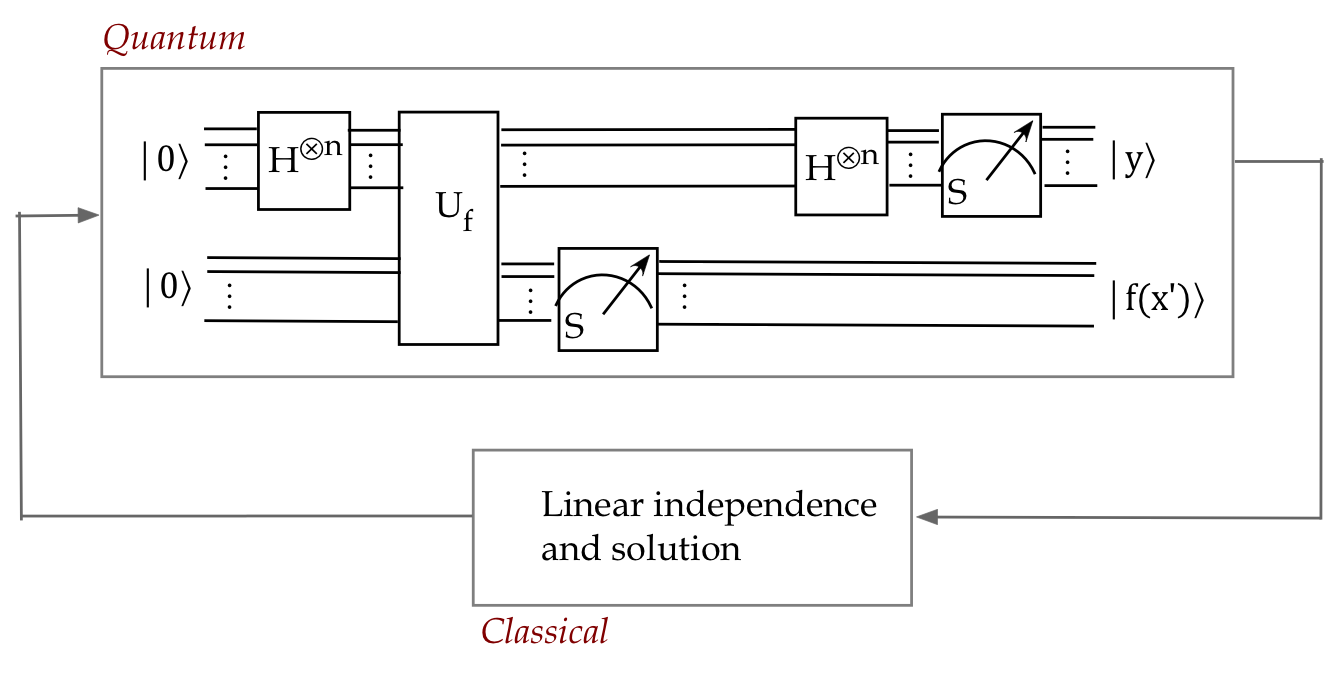
\includegraphics[width=5in]{notes/figs/n11/23simon3.png}
            \caption{Simon's algorithm circuit}
        \label{fig:23simon3}
    \end{figure}
    
    Trials are repeated until $n$ independent equations $c \cdot y_{i}=20$ are found. The equations are classically solved for $c$. With very high probability, only $O(n)$ trials are needed, in comparison to an exponential classical solution. What do we learn from this problem and algorithm?   This algorithm exemplifies how a combination of quantum-and-classical can iteratively solve a problem. The problem is no less contrived than the others. However, this problem provided insight that led to Shor's algorithm.

\end{document}